% RP^2 as a disk with antipodal boundary points identified (two half-arcs).
% Source: book/tex/topology/constructions.tex (§ Real projective space).
\documentclass[border=2mm]{standalone}
\usepackage{tikz}
\usepackage{amssymb}
\usetikzlibrary{arrows.meta,decorations.markings}
\tikzset{midarr/.style={decoration={markings,
  mark=at position 0.5 with {\arrow{Latex[length=2mm]}}},postaction={decorate}}}
\begin{document}
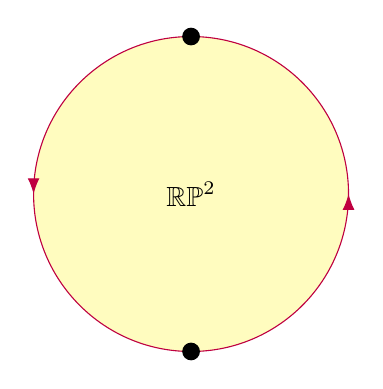
\begin{tikzpicture}[scale=2]
  \fill[yellow!25] (0,0) circle (1);
  \draw[purple, midarr] (-90:1) arc (-90:90:1);  % right half
  \draw[purple, midarr] (90:1) arc (90:270:1);   % left half
  \fill (0,1) circle (1.6pt);
  \fill (0,-1) circle (1.6pt);
  \node at (0,0) {$\mathbb{RP}^2$};
\end{tikzpicture}
\end{document}
